\chapter{Dopasowanie kształtów}

Lokalnie pokrewne fragmenty obrazu (ang. Local Affine Frames) łączone w pary,
służą do ustalania korespondencji pomiędzy dwoma obrazami. Sposób opisu tych
regionów wpływa na jakość wyników algorytmu dopasowującego. Ze względu na nasze
wymagania, będziemy potrzebowali takiego sposobu reprezentacji, aby w jak
najmniejszym stopniu wpływały na nią zmiana skali oraz perspektywy obrazu. Z
pomiarów opublikowanych w "Shape Guided Maximally Stable Extremal
Region (MSER) Tracking" \cite{mser_tracking} wynika, że kontury znacznie
dokładniej niż elipsy opisują badane regiony i jednocześnie nie wymagają dużych
zasobów do obliczenia wyznacznika podobieństwa. Najszybszym obecnie algorytmem
do dopasowania kształtów jest IS-Match przedstawiony przez M. Donoser et al.
\cite{ismatch}.

Dodatkowym atutem tego rozwiązania jest możliwość wyznaczenia miary
podobieństwa konturów na podstawie ich fragmentów, wyrażoną przez optimum
Pareta.

\section{Opis konturu}

Algorytmy dopasowania kształtów możemy podzielić na dwie kategorie: globalne i
lokalne. Podejście globalne porównuje całości konturów i działa pod warunkiem
braku znaczących deformacji takich jak zgięcia, częściowe przysłonięcia itp.
Dopasowanie lokalne pozwala na dopasowanie fragmentów konturu, ale osiąga
gorsze rezultaty przy dopasowaniu całości. Algorytm IS-Match (ang. Integral
Shape Match) posiada cechy obu tych podejść. Tak jak przy dopasowaniu
globalnym, kształt reprezentuje się za pomocą punktów próbkowanych z konturu.
Opis konturu składa się natomiast z kątów siecznych $\alpha$, które zawierają w sobie
zarówno lokalne jak i globalne cechy, dzięki czemu możliwe jest dopasowanie
różnych, przekształconych, zmodyfikowanych, a nawet częściowych, wersji
konturu.

Deskryptor jest oparty o kąty $\alpha_{ij}$, które określają układ pomiędzy
punktami konturu. Kąt $\alpha_{ij}$ znajduje się pomiędzy sieczną z
referencyjnego punktu $P_{i}$ do punktu $P_{j}$ oraz sieczną z punktu $P_{j}$
do punktu $P_{j-\Delta}$, gdzie $i$ oraz $j$ przyjmują wartości od $1$ do $N$
czyli liczby punktów w konturze, a $\Delta$ jest parametrem. Taki sposób opisu
pozwala pozostać obojętnym na zmianę skali czy rotacje, przy której żaden kąt
się nie zmienia.

\begin{figure}[h!] \centering
  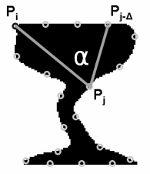
\includegraphics[]{images/alpha.png}
  \caption{ Kąt $\alpha_{ij}$. Źródło: \cite{ismatch} } \end{figure}

Po obliczeniu wszystkich kątów otrzymujemy macierz o rozmiarze $N \times N$,
opisującą nasz kontur. Elementy na diagonali zawsze mają wartość zero, gdyż
odpowiadają kątowi, którego oba ramiona kończą się w tym samym punkcie. Cechy
lokalne konturu zawarte są bliżej diagonali, a globalne dalej. Nie ma znaczenia
od którego punktu zaczniemy iterację, ponieważ macierz jest cykliczna i możemy
ją przesuwać wzdłuż diagonali.

Nie jest istotne czy próbkowane punkty na konturze będą oddalone od siebie o
stałą odległość, czy dla każdego konturu będzie to stała liczba punktów
niezależnie od ich wielkości. Oba podejścia mają inne cechy i trudno
stwierdzić, który z tych opisów jest lepszy. W dalszej części pracy założyłem,
że rozmiar deskryptora jest zależny od długości obwodu konturu.

\begin{figure}[h!] \centering \subfloat[Kształt
  1]{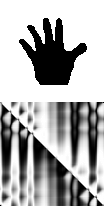
\includegraphics[width=0.25\textwidth]{images/hand.png} \label{hand}}
  \subfloat[Kształt 2]{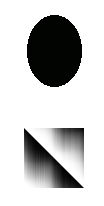
\includegraphics[width=0.25\textwidth]{images/egg.png}
  \label{egg}} \caption{Graficzna reprezentacja macierzy deskryptorów. Kolor
  czarny odpowiada kątowi $0^\circ$, kolor biały kątowi $360^\circ$. Kąty
  liczone są co trzeci piksel. Przy stałej liczbie próbek skomplikowanego
  konturu \ref{hand}, istaniałoby ryzyko że próba będzie zbyt mała, a kształt
  fałszywie uproszczony. W przypadku konturu \ref{egg} ilość próbek nie ma
  większego znaczenia.} \end{figure}

\section{Odnajdywanie podobieństw}

Załóżmy, że chcemy porównać dwa kształty. Naszym celem będzie znalezienie
podobnych do siebie fragmentów konturów, reprezentowanych przez macierze
kątowe: $A_{1}$ o rozmiarze $M \times M$ i $A_{2}$ o rozmiarze $N \times N$,
gdzie $M \leq N$.  Matematycznie oznacza to znalezienie takiego bloku o
rozmiarze $r \times r$, zaczynającego się w punkcie $A_1(s,s)$ (leżącego na
diagonali tej macierzy), który zwróci różnicę kątową $D_{\alpha}(s,m,r)$, z
blokiem $A_{2}(m,m)$, poniżej zadanej wartości progowej. 

% \begin{equation}
%   D_{\alpha}(s,m,r) = \frac{1}{r^2} \sum_{i=0}^{r-1} \sum_{j=1}^{r-1} [A_{1}(s+i, s+j) - A_{2}(m+i, m+j)]^2.
%   \label{eq:wzor1}
% \end{equation}

Ponieważ musimy rozważyć każdy, dowolnie duży blok, zaczynający się w dowolnym
miejscu na diagonali, metoda iteracyjnego odejmowania wszystkich kątów
wymagałaby zbyt dużo mocy obliczeniowej i nie jest stosowana.

Efektywniejszą metodą obliczenia wyznacznika podobieństwa dla wszystkich trzech
parametrów $s,m,r$ jest budowa $N$ macierzy różnicowych (ang. descriptor
difference matrices) $M_{D}^{n}$ o rozmiarze $M \times M$, które dopasowują
kolejne punkty konturu $A_{1}$ (parametr s):

\begin{equation}
  M_{D}^{n} = A_{1}(1: M, 1: M) - A_{2}(n: n+M-1, n:n+M-1).
\end{equation}

Jeżeli naszym celem jest uzyskanie tylko jednej miary podobieństwa, która
określi to, jak dobrze można dopasować cały mniejszy kontur, do tak samo dużego
fragmentu większego konturu, to będzie nią średnia wartość wszystkich elementów
macierzy $M_{D}^{n}$. Ponieważ dla naszych celów jest to w zupełności
wystarczająca informacja, w dalaszej części pracy zostanie omówiony algorytm
właśnie tej miary.

W przeciwnym razie, dla każdej macierzy różnicowej, należy szukać iteracyjnie
optymalnych wartości parametrów $m$ i $r$. Ponieważ dla jednej wartości
parametru $s$ możemy uzyskać wiele pasujących fragmentów konturu, należy
zwrócić wszystkie z nich. Te dane stanowią później podstawę do obliczenia
optimum Pareto, za pomocą miar podobieństwa i niepodobieństwa, szczegółowo
opisanych przez Bronsteina i innych \cite{partial_similarity}.

Ponieważ przekształcenia inne niż geometryczne nie są przewidziane, liczenie
współczynnika podobieństwa biorącego pod uwagę takie nietypowe przekształcenia,
nie zostało zaimplementowane i wszystkie uzyskane przeze mnie wyniki bazują na
uproszczonej wersji algorytmu.

\section{Algorytm}

\subparagraph{Struktury danych} 

\begin{itemize} \item Kontur jest tablicą pikseli reprezentowanych przez
    indeks: $x + y*width$. \item Deskryptor jest jednowymiarową tablicą
    zawierającą wartości cosinus kątów $\alpha$ (wartości z przedziału od -1 do 1).
\end{itemize}

\subparagraph{Algorytm opisu konturu}: Funkcja na wejściu przyjmuje kontur i
parametr $\Delta$, a zwraca macierz deskryptora $A$.  

\begin{enumerate} \item Znajdź $N \times N$ dwuelementowych wariacji z
    powtórzeniami, pikseli konturu. \item Dla każdej pary znajdź cosinus kąta
    pomiędzy pierwszym punktem $P_{i}$, drugim punktem $P_{j}$ i punktem
    $P_{j-\Delta}$, podany wzorem: 

\begin{equation}
  A_{i,j} = \frac{c^2 - a^2 - b^2}{-2ab}.
\end{equation}

 Wartości $a$, $b$ i $c$ to długości odcinków pomiędzy punktami $P_i$ i $P_j,$
 $P_j$ i $P_{j-\Delta}$ oraz $P_{j-\Delta}$ i $P_i$. \end{enumerate}

\subparagraph{Algorytm dopasowania konturów}: Funkcja na wejściu przyjmuje dwa
deskryptory konturów. Zwraca współczynnik ich podobieństwa oraz indeks punktu,
na większym z tych dwóch konturów, który odpowiada pierwszemu punktowi na
mniejszym konturze.

\begin{enumerate} \item Przypisz do zmiennej $A1$ mniejszy z dwóch deskryptorów
    o wymiarach $M \times M$, a $A2$ większy o rozmiarze $N \times N$. \item
    Niech $n = 0$ będzie indeksem elementów na diagonali macierzy $A2$. \item
    Wyznacz macierz różnicową $M_{D}^n$ pomiędzy macierzą $A1$, a macierzą tej
    samej wielkości, zaczynającej się w punkcie $A2_{n,n}$. Jeżeli wiersz lub
    kolumna wykracza poza zakres macierzy $A2$, zastąp je elementem o wartości
    różnicy z dzielenia danego indeksu przez $N$. \item Oblicz sumę wszystkich
    elementów macierzy i podziel ją przez $M^2$, liczbę wszystkich elementów.
  \item Zwiększ $n$ o jeden. Jeżeli $n < N$, przejdź do punktu 3. \item Zakończ
    zwracając parę: \textit{offset} i \textit{min}.  \end{enumerate}

\section{Złożoność obliczeniowa}

Złożoność obliczeniowa algorytmu dopasowania \cite{ismatch} zależy od liczby
punktów opisujących kontury i wynosi $O(nm)$. Ten sam kontur można jednak
opisać mniejszą lub większą liczbą punktów, co będzie skutkować zwieszeniem
szybkości lub dokładności algorytmu.
